\documentclass[a4paper,10pt]{article}
\usepackage[utf8]{inputenc}
\usepackage{xlop}
\usepackage[]{amsmath}
\usepackage[]{url}
\usepackage{graphicx}

\usepackage[linesnumbered,vlined,ruled]{algorithm2e}
    \usepackage[left=0.7in, right=0.7in, top=0.5in, bottom=0.43in]{geometry}

\title{Method of Multiplication of two 2- digit numbers}
\author{Anmol Porwal}
\date{5 March 2017 }
\begin{document}

\maketitle
 \begin{center}
\textbf{ABSTRACT}
 \end{center}
Multiplication is a procedure which every human being encounters on a daily basis. Of course, we have calculators for it, but using out calculators for every single product is a cumbersome process if we have to do it for a list of numbers. So, in this paper I will be discussing some faster methods to multiply two 2-digit numbers. The ideas in this article are from Atharvaveda \cite{Atharvaveda}. 
\section{\textbf{METHOD}}
The two numbers can be entirely different (having no co-relation between them). I will be stating methods only for two specific cases.

\subsection {Case 1} \label{casea}
The first two digits are the same and the last two add up to ten.
\newline
Let us see a few examples for this case.
\newline
Example 1 : Numbers are 66 and 64
\begin{center}
\opmul{66}{64}\qquad
\end{center}
Example 2 : Numbers are 31 and 39
\begin{center}
\opmul{31}{39}\qquad
\end{center}
How to do it fastly - \newline
For example 1 - write 6$\times$(6+1):6$\times$(4) = 42:24 , i.e. , 4224 \newline
For example 2 - write 3$\times$(3+1):1$\times$(9) = 12:09 , i.e. , 1209 \newline
\begin{figure}
    \centering
    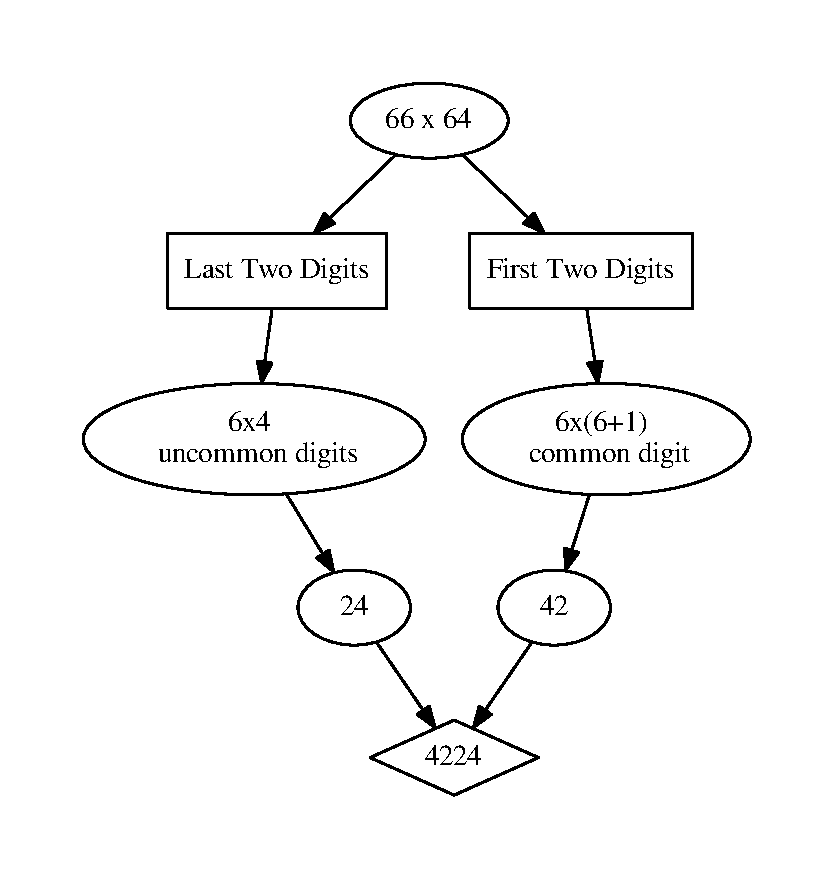
\includegraphics[width=0.65\textwidth]{figure.pdf}
    \caption{Case1:Example1: 66 x 64 }
    \label{fig:my_label}
\end{figure}
So, in general if you have numbers like $ab$ and $ac$ where $b$ + $c$ = 10. Then the result of $ab \times ac$ will be $a\times(a+1)$ : $b\times(c)$. The expression on left of ":" will always be of two digits and on the right of ":" as well.

The pseudo code for the algorithm in this case is given below.

\begin{algorithm}[H]
m and n are the inputs \\
$a \gets m/10$ \\
$d \gets a\times(a+1)$ \\
$b \gets m\%10$ \\
$c \gets n\%10$ \\
$e \gets b\times c$ \\
\If{d/10 is not zero and e/10 is not zero }{print de}
\ElseIf{d/10 is not zero and e/10 is zero}{print d0e}
\ElseIf{d/10 is  zero and e/10 is not zero}{print 0de}
\ElseIf{d/10 is  zero and e/10 is zero}{print 0d0e}
\caption{Multiply for \ref{casea}}
\end{algorithm}


\subsection{Case 2} \label{caseb}
The first two digits add up to 10 and the last two are same.
\newline
Let us see a few examples for this case.
\newline
Example 1 : Numbers are 34 and 74
\begin{center}
\opmul{34}{74}\qquad
\end{center}
Example 2 : Numbers are 90 and 10
\begin{center}
\opmul{10}{90}\qquad
\end{center}
How to do it fast - \newline
For example 1 - write 3$\times$7 + 4:4$\times$4 = 25:16 , i.e. , 2516 \newline
For example 2 - write 9$\times$1 + 0:0$\times$0 = 90:00 , i.e. , 9000 \newline
\begin{figure}
    \centering
    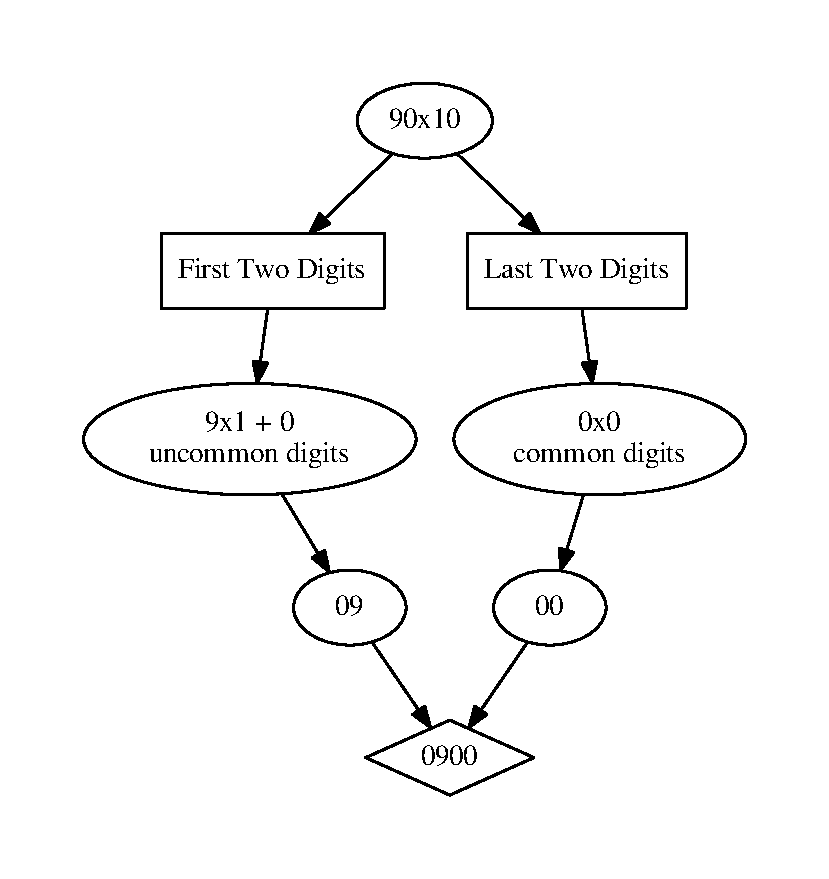
\includegraphics[width=0.68\textwidth]{figure1.pdf}
    \caption{Case2:Example2: 90 x 10 }
    \label{fig:my_label1}
\end{figure}
So, in general if you have numbers like $ab$ and $cb$ where $a$ + $c$ = 10. Then the result of $ab \times cb$ will be $a\times c $ + $b$ : $b \times b$. The expression on left of ":" will always be of two digits and on the right of ":" as well. \\ \\
The pseudo code for the algorithm in this case is given below

\begin{algorithm}[H] 
$a \gets m/10$ \\
$b \gets m\%10$ \\
$c \gets n/10$ \\
$d \gets a\times c + b$ \\
$e \gets b\times b$ \\
\If{d/10 is not zero and e/10 is not zero }{print de}
\ElseIf{d/10 is not zero and e/10 is zero}{print d0e}
\ElseIf{d/10 is  zero and e/10 is not zero}{print 0de}
\ElseIf{d/10 is  zero and e/10 is zero}{print 0d0e}
\caption{Multiply for \ref{caseb} \footnote{The algorithm is from \cite{Corman}}}
\end{algorithm}

\section{SUMMARY}

\begin{table}[ht]
\centering
\caption{Methods}
\begin{tabular}{|c||c|}

\hline
    Cases & Method \\
    \hline
    Right digit(b and c) sum is 10 and Left digits(a) are identical & a$\times$(a+1) : b$\times$c \\
    Right digit (b) is identical and Left digits(a and c) sum is 10 & a$\times$c+b : b $\times$ b \\
   \hline
   \end{tabular}
   \label{method}
    \end{table}

\section{\textit{Is it really faster ?}}
It is quite evident form the procedure listed out in both the cases that it is quite easy and amazingly faster. We are very fast in multiplying single-digit numbers ( because in middle school, we are told again and again to memorize tables). And in the mehtods we are essentially multiplying single digit and a bit of addition, which is obviously trivial. Otherwise in the conventional approach, we have to work out \textbf{four single digit multiplication} and an \textbf{addition of two 3-digit numbers}. Thus, the methods are quite faster than conventional method.

\section{\textit{Why it works}}

\subsection{\textbf{CASE 1} - \textbf{Proof}}


Let the two numbers be $10a$ + $b$ and $10a$ + $c$. 
\begin{equation}
\label{eq1}
    (10a + b)\times(10a + c)=100\times a \times c + 10\times a(b+c) + b\times c
\end{equation}
We know that $b+c = 10$,hence substitute $b+c$ in \ref{eq1}, we get
\begin{equation}
100\times a \times c + 10\times a(b+c) + b\times c=100\times a \times c + 10\times 10\times a + b\times c 
\end{equation}
Further simplifying,

\begin{align}
100\times a \times c + 100\times a + b\times c &= 100\times (a \times c + a) + b\times c \\
%\end{equation}
%The rightmost expresion in (2) can be re-arranged as
%\begin{equation}
 100\times (a \times c + a) + b\times c &= 100\times a \times (c + 1) + b\times c
\end{align}


Observe that $a \times (c + 1)$ is always less than or equal to 90 as $a$ and $c$ are single-digit numbers. Also, $b \times
c $ is always less than or equal to 81. Hence, $a \times (c + 1)$ occupy the first two digits of the number and $b\times c$ take the last two digits. \footnote{If $a \times (c + 1)$ or $b\times c$ are single digit , then add 0 on left of the numbers (as shown in Example 1 of \ref{casea})} \newline
$NOTE$ : If $a \times (c + 1)$ or $b\times c$ are single digit , then add 0 on left of the numbers (as shown in Example 1).

\subsection{\textbf{CASE - 2} - \textbf{Proof}}


Let the two numbers be $10a$ + $b$ and $10c$ + $b$. 
\begin{equation}
\label{eq2}
    (10a + b)\times(10c + b)=100\times a \times c + 10\times b(a+c) + b\times b
\end{equation}
We know that $a+c = 10$,hence substitute $a+c$ in \ref{eq2}, we get
\begin{align}
100\times a \times c + 10\times b(a+c) + b\times b &= 100\times a \times c + 10\times 10\times b + b\times b 
\\
100\times a \times c + 100\times b + b\times b 
&= 100\times (a \times c + b) + b\times b
\end{align}

Observe that $a \times c + b$ is always less than or equal to 90 as $a$, $b$ and $c$ are single-digit numbers. Also, $b \times b $ is always less than or equal to 81. Hence, $a \times c + b$ occupy the first two digits of the number and $b\times b$ take the last two digits.\footnote{If $a \times c + b$ or $b\times b$ are single digit , then add 0 on left of the numbers (as shown in Example 2 of \ref{caseb})} \newline
$NOTE$ : If $a \times c + b$ or $b\times b$ are single digit , then add 0 on left of the numbers (as shown in Example 1).

\section{Generalization to more number of digits}
A natural question arises that can we apply this kind of method for 3-digit or 4-digit numbers? The answer is \textbf{YES}. In fact we can apply this method for any number of digits.
First let's look at an example-
\newline
Example Case1-
\begin{center}
\opmul{123}{177}\qquad
\end{center}
So, this has first digit same and remaining 2-digit quantities sum up to 100. As we did in \ref{casea}, we can do same here. 1 $\times$ (1+1) : 23 $\times$ 77 ,i.e, 021771 \newline
The intuition behind generalization in case 1: Let the number of digits be n. break each number in 2 parts the first digit and the rest of n-1 digits so if number is N = fZ where f is $1^{st}$ digit and Z is rest of n-1 digits then it can be represented as f x $10^{n-1}$ + Z so product would be ( $Z_1$ x $Z_2$  + $f^2$ x $10^{2n-2}$ +  ($Z_1$ + $Z_2$) x f x $10^{n-1}$) now since $Z_1$ + $Z_2$ = $10^{n-1}$ the product becomes ($Z_1$ x $Z_2$  + f x (f+1) x $10^{2n-2}$) =  f x (f+1) : $Z_1$ x $Z_2$.               

Example Case2-
\begin{center}
\opmul{325}{685}\qquad
\end{center}
So, this has sum of first two digit as 100 and remaining digit is same in both numbers. As we did in \ref{caseb}, we can do same here 32$\times$68 + 10$\times$5 : 5$\times$5 , i.e. , 2176+50:25 = 222625. \emph{Notice the extra 10 being multiplies here}.\newline
The intuition behind generalization in case 2: Let the number of digits be n. break each number in 2 parts the first n-1 digits and the last digit. So if number is N = Zl where Z represents first n-1 digits and l is last digit then it can be represented as 10$\times$Z + l so product would be ( $100\times (Z_1\times Z_2) + 10\times  (Z_1+Z_2) \times l + l^2$ ) now since $Z_1 + Z_2 = 10^{n-1}$ the product becomes ( $100\times ((Z_1\times Z_2) + 10^{n}\times l) + l^2$ ) = $Z_1\times Z_2 + 10^{n}\times l$ : $l^2$.

\bibliographystyle{unsrt}
\bibliography{bib}

\end{document}
